\subsection{Quadratic Functions}
Quadratic functions are those in the form of $y=x^2$. They have a degree of 2. The shape of the graph is known as a parabola.

\subsubsection{Equations and Terminology}
Terminology:\\
The vertex is the lowest or highest point of the parabola (where it changes directions.)\\
The axis of symmetry is the vertical line that divides the parabola in half, going through the vertex.\\
A parabola will always have 1 y-intercept and either 0, 1, or 2 x-intercepts.\\
The domain of a parabola is $x\in\mathbb{R}$\\
The range of a parabola is dependent on which way it opens and the height of the vertex.\\
\\
\centerline{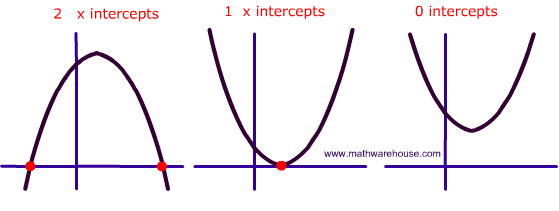
\includegraphics[scale = 0.6]{Images/PreCalcPictures/ParabolaSolutions.png}}

Vertex Form: $y=a(x-p)^2+q$\\
$a$ determines how steep the parabola is. Larger values make it steeper and smaller values make it rise more gradually. If $a$ is positive, the parabola opens up. If $a$ is negative, the parabola opens down. $p$ determines how far to the right of the origin the vertex will be located. $q$ determines how far above the origin the vertex will be located.\\
This form is useful for graphing because you know exactly where the vertex is and how fast the slope is rising.\\
\\
Standard Form: $y=ax^2+bx+c$\\
$a$ determines how steep the parabola is and which way it opens. $c$ is the y-intercept.\\
This form is useful for solving quadratic equations.\\
\\
Converting between forms:\\
To convert vertex form to standard form, you simply need to expand the squared term inside the brackets.\\
To convert from standard form to vertex form, you can either use the conversion formulas of $p=-\dfrac{b}{2a}$ and $q=c-\dfrac{b^2}{4a}=c-ap^2$ or you can use completing the square method. Completing the square involves adding and subtracting a value in order to create a perfect square trinomial.\\
Ex: $x^2+6x+5$
\begin{align*}
    &x^2+6x+5+9-9\\
    &(x^2+6x+9)-4\\
    &(x+3)^2-4
\end{align*}
Ex2: $4x^2-32x-23$
\begin{align*}
    &4(x^2-8x)-23\\
    &4(x^2-8x+16)-23-4(16)\\
    &4(x^2-4)^2-87
\end{align*}

\subsubsection{Solving Quadratic Equations}
Solving by Factoring:
First we must set $y=0$. Then we can factor our quadratic. We will have two terms. At least one of the terms must be equal to zero in order to give an answer of zero so to solve, we can set both terms equal to zero and solve for $x$.\\
Ex: $y=x^2+4x-21$
\begin{align*}
    0=&(x+7)(x-3)\\
    0=&(x+7)\Ra x=-7\\
    0=&(x-3)\Ra x=3
\end{align*}
\\
Solving by Completing the Square:\\
Ex: $y=x^2-6x+7$
\begin{align*}
    y=&x^2-6x+9+7-9\\
    y=&(x-3)^2-2\\
    0=&(x-3)^2-2\\
    2=&(x-3)^2\\
    x-3=&\pm \sqrt{2}\\
    x=&3\pm \sqrt{2}
\end{align*}
\\
The Quadratic Formula:\\
Derivation:\\
If there is no horizontal shift, a quadratic will take the form $y=ax^2+q$ and solving the quadratic is easy. We can make any quadratic take this form by applying a horizontal translation, shifting the quadratic by the location of the vertex. So we set $x=x_s-\frac{b}{2a}$. This will allow us to solve for any quadratic.
\begin{align*}
    0=&ax^2+bx+c\\
    0=&a\left(x_s-\frac{b}{2s}\right)^2+b\left(x_s-\frac{b}{2a}\right)+c\\
    0=&\left(x_s-\frac{b}{2s}\right)^2+\frac{b}{a}\left(x_s-\frac{b}{2a}\right)+\frac{c}{a}\\
    0=&x_s^2-\frac{b}{a}x_s+\frac{b^2}{4a^2}+\frac{b}{a}x_s+\frac{c}{a}\\
    x_s^2=&\frac{b^2}{4a^2}-\frac{c}{a}=\frac{b^2-4ac}{4a^2}\\
    x_s=&\pm\frac{\sqrt{b^2-4ac}}{2a}\\
    x=&x_s-\frac{b}{2a}=-\frac{b}{2a}\pm\frac{\sqrt{b^2-4ac}}{2a}\\
    x=&\frac{-b\pm\sqrt{b^2-4ac}}{2a}
\end{align*}
*A similar derivation could be done using the complete the square method.\\
This formula allows us to solve any quadratic equation. It also has a property that allows us to deduce how many solutions a quadratic will have without actually solving it. This is done using the discriminant (the part under the square root).\\
If $b^2-4ac>0$ there are 2 real solutions\\
If $b^2-4ac=0$ there is 1 real solution\\
If $b^2-4ac<0$ there are no real solutions\\
\\
Systems of Quadratic Equations:\\
To find the point(s) where two quadratics intersect, we can use substitution for $y$ and set the two equations equal to each other. This gives a new quadratic and will give the points of intersection.\\
Ex: $\left\{\begin{matrix} y=3x^2-x-2\\
y=6x^2+4x-4 \end{matrix}\right.$
\begin{align*}
    3x^2-x-2=&6x^2+4x-4\\
    0=&3x^2+5x-2\\
    0=&(3x-1)(x+2)\\
    0=&(3x-1)\Ra x=\frac{1}{3}\\
    0=&(x+2)\Ra x=-2
\end{align*}

\subsubsection{Quadratic Inequalities}
Because a quadratic can have two x-intercepts, it can have two places it switches from positive to negative so quadratic inequalities are often bounded by two numbers.\\
We can break it up into a series of linear cases based on factors.\\
Ex: $(x+3)(x-2)\geq 0$\\
$x+3\geq 0\Ra x\geq -3$\\
\centerline{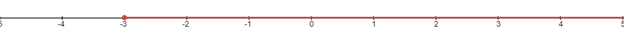
\includegraphics[]{Images/PreCalcPictures/Inequality1.png}}
$x-2\geq 0\Ra x\geq 2$\\
\centerline{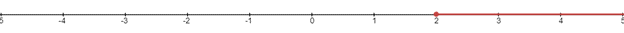
\includegraphics[]{Images/PreCalcPictures/Inequality2.png}}
$(x+3)(x-2)\geq 0\Ra x\leq -3\,\mathrm{or}\,x\geq 2$\\
\centerline{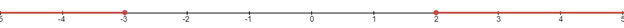
\includegraphics[]{Images/PreCalcPictures/Inequality3.png}}
This method of lining up the number line graphs works for all polynomials and even rational expressions to solve for difficult inequalities.